\section{Knowledge Assessment}

% categories
\begin{frame}{Fact-Completion Dataset}
\begin{table}[t!]
    \centering
    \begin{tabular}{l|l}
        \hline\hline
        \textbf{Category} & \multicolumn{1}{c}{\textbf{Description}} \\\hline
        \textsf{nation-capital}     &   The capital of <country $x$> is <$y$> \\
        \textsf{person-birthloc}    &   <person $x$> was born in <$y$> \\
        \textsf{person-birthdate}   &   <person $x$> was born on <$y$> \\
        \textsf{person-spouse}      &   <person $x$> is married to <$y$> \\
        \textsf{city-state}         &   <city $x$> is a city in the state of <$y$> \\
        \textsf{book-author}        &   <book $x$> is a book that was written by <$y$> \\
        \hline\hline
    \end{tabular}
\end{table}

Descriptions of the Fact Completion dataset for each category. Many of the following experiments are based 600 sentences from these categories (100 sentences each).
\end{frame}

\subsection{Into the guts of KnowBERT}

\begin{frame}{Into the guts of the KAR mechanism}
Recall this fella,
\begin{figure}
    \centering
    \includegraphics[width=1\textwidth]{graphics/kb/Knowbert_KAR_mechanism.pdf}
\end{figure}
\pause
We focus know specifically on the \stepbox{DTU_yellow}{Mention Spans}, the \stepbox{DTU_purple}{Entity Linking}, and the \stepbox{DTU_blue}{Recontextualisation} steps.
\end{frame}

% \begin{frame}{The guts of KAR: Barack Obama}
%     \KARPLOT{2}
% \end{frame}
% \begin{frame}{The guts of KAR: Barack Obama (Cont'd)}
%     \begin{table}[t!]
\tiny
\centering
\begin{tabular}{|p{2.4cm}|p{2.8cm}c|p{2.8cm}c|}
\hline
\multirow{3}{*}{\textbf{Candidate Spans}} & \multicolumn{4}{c|}{\textsf{barack obama is married to michelle obama . }} \\
& \multicolumn{2}{c}{Priors (top-2)} & \multicolumn{2}{c|}{Norm. EL Scores (top-2)} \\ \cline{2-5}
& \multicolumn{1}{c|}{\textsf{ent}} & $p(\mathsf{ent})$ & \multicolumn{1}{c|}{\textsf{ent}} & $\psi_{m,k}$ \\ \hline 
\multicolumn{5}{c}{\textbf{\textsf{Wiki}}}\\
\hline
\multirow{2}{*}{\textsf{barack}}& Barack Obama & 0.53 & 2000 Camp David Summit & 0.07\\ 
& Barack (brandy) & 0.15 & Barack Obama & 0.07\\\hline 
\multirow{2}{*}{\textsf{barack obama}}& Barack Obama & 0.54 & Barack Obama & 0.06\\ 
& Barack Obama, Sr. & 0.09 & 2009 Nobel Peace Prize & 0.04\\\hline 
\multirow{2}{*}{\textsf{obama}}& Barack Obama & 0.47 & Community organizing & 0.03\\ 
& Obama, Fukui & 0.05 & Presidency of Barack Obama & 0.03\\\hline 
\multirow{2}{*}{\textsf{married}}& Marriage & 0.32 & Jennifer Siebel & 0.03\\ 
& Same-sex marriage in California & 0.13 & Kateryna Yushchenko & 0.03\\\hline 
\multirow{2}{*}{\textsf{michelle}}& Michelle Obama & 0.40 & Michelle Lang & 0.03\\ 
& Michelle (song) & 0.24 & Michelle Pfeiffer & 0.03\\\hline 
\multirow{2}{*}{\textsf{michelle obama}}& Michelle Obama & 1.00 & Michelle Obama & 0.60\\ 
& Celebrity (game) & 0.00 & Celebrity (game) & 0.40\\\hline 
\multirow{2}{*}{\textsf{michelle obama .}}& Michelle Obama & 1.00 & Michelle Obama & 1.00\\ 
& N/A & 0.00 & N/A & 0.00\\\hline 
\multirow{2}{*}{\textsf{obama}}& Barack Obama & 0.47 & Barack Obama citizenship conspiracy theories & 0.03\\ 
& Obama, Fukui & 0.05 & Community organizing & 0.03\\\hline 
\multicolumn{5}{c}{\textbf{\textsf{Wordnet}}}\\
\hline
\multirow{2}{*}{\textsf{is}}& be.v.01 & 0.64 & be.v.01 & 1.00\\ 
& be.v.02 & 0.18 & be.v.03 & 0.00\\\hline 
\multirow{2}{*}{\textsf{married}}& marry.v.01 & 0.94 & marry.v.01 & 1.00\\ 
& marry.v.02 & 0.06 & marry.v.02 & 0.00\\\hline 
\end{tabular}
\end{table}
% \end{frame}

\begin{frame}{The guts of KAR: Kobe Bryant}
    \KARPLOT{1}
\end{frame}
\begin{frame}{The guts of KAR: Kobe Bryant (Entities)}
    \begin{table}[t!]
\tiny
\centering
\begin{tabular}{|p{2.4cm}|p{2.8cm}c|p{2.8cm}c|}
\hline
\multirow{3}{*}{\textbf{Candidate Spans}} & \multicolumn{4}{c|}{\textsf{kobe bryant was born in philadelphia . }} \\
& \multicolumn{2}{c}{Priors (top-2)} & \multicolumn{2}{c|}{Norm. EL Scores (top-2)} \\ \cline{2-5}
& \multicolumn{1}{c|}{\textsf{ent}} & $p(\mathsf{ent}|m)$ & \multicolumn{1}{c|}{\textsf{ent}} & $\psi_{m,k}$ \\ \hline 
\multicolumn{5}{c}{\textbf{\textsf{Wiki}}}\\
\hline
\multirow{2}{*}{\textsf{kobe}}& Great Hanshin earthquake & 0.26 & Kobe Bryant & 0.09\\ 
& Kobe Bryant & 0.22 & Derek Fisher & 0.09\\\hline 
\multirow{2}{*}{\textsf{kobe bryant}}& Kobe Bryant & 0.56 & Kobe Bryant & 0.26\\ 
& Kobe Bryant sexual assault case & 0.15 & Los Angeles Lakers & 0.25\\\hline 
\multirow{2}{*}{\textsf{bryant}}& William Cullen Bryant & 0.10 & Bryant, Minneapolis & 0.03\\ 
& Bryant, Humboldt County, California & 0.10 & Kobe Bryant & 0.03\\\hline 
\multirow{2}{*}{\textsf{born}}& Nativity of Jesus & 0.70 & Frank Zamboni & 0.03\\ 
& Michael Savage & 0.02 & Ingvar Kamprad & 0.03\\\hline 
\multirow{2}{*}{\textsf{philadelphia}}& Philadelphia & 0.70 & Philadelphia & 0.05\\ 
& Philadelphia (film) & 0.03 & Philadelphia Eagles & 0.03\\\hline 
\multicolumn{5}{c}{\textbf{\textsf{Wordnet}}}\\
\hline
\multirow{2}{*}{\textsf{kobe}}& kobe.n.01 & 1.00 & kobe.n.01 & 1.00\\ 
& N/A & 0.00 & N/A & 0.00\\\hline 
\multirow{2}{*}{\textsf{was}}& be.v.01 & 0.64 & be.v.01 & 0.99\\ 
& be.v.02 & 0.18 & equal.v.01 & 0.01\\\hline 
\multirow{2}{*}{\textsf{born}}& bear.v.01 & 0.24 & give birth.v.01 & 1.00\\ 
& give birth.v.01 & 0.18 & wear.v.02 & 0.00\\\hline 
\multirow{2}{*}{\textsf{in}}& in.r.01 & 0.69 & in.s.03 & 1.00\\ 
& inch.n.01 & 0.14 & in.s.01 & 0.00\\\hline 
\multirow{2}{*}{\textsf{philadelphia}}& philadelphia.n.01 & 1.00 & philadelphia.n.01 & 1.00\\ 
& N/A & 0.00 & N/A & 0.00\\\hline 
\end{tabular}
\end{table}
\end{frame}


\begin{frame}{The guts of KAR: The city of Kobe}
    \KARPLOT{0}
\end{frame}
\begin{frame}{The guts of KAR: The city of Kobe (Entities)}
    \vspace{-0.15cm}
    \begin{table}[t!]
\tiny
\centering
\begin{tabular}{|p{2.4cm}|p{3.2cm}c|p{3.2cm}c|}
\hline
\multirow{3}{*}{\textbf{Candidate Spans}} & \multicolumn{4}{c|}{\textsf{kobe is a city in the state of japan . }} \\
& \multicolumn{2}{c}{Priors (top-2)} & \multicolumn{2}{c|}{Norm. EL Scores (top-2)} \\ \cline{2-5}
& \multicolumn{1}{c|}{\textsf{ent}} & $p(\mathsf{ent})$ & \multicolumn{1}{c|}{\textsf{ent}} & $\psi_{m,k}$ \\ \hline 
\multicolumn{5}{c}{\textbf{\textsf{Wiki}}}\\
\hline
\multirow{2}{*}{\textsf{kobe}}& Great Hanshin earthquake & 0.26 & Great Hanshin earthquake & 0.12\\ 
& Kobe Bryant & 0.22 & Kobe Bryant & 0.09\\\hline 
\multirow{2}{*}{\textsf{city}}& City & 0.45 & Cities of the ancient Near East & 0.03\\ 
& City status in the United Kingdom & 0.08 & Urban areas in Sweden & 0.03\\\hline 
\multirow{2}{*}{\textsf{state}}& Political divisions of the United States & 0.50 & Michigan & 0.03\\ 
& U.S. state & 0.10 & States of Brazil & 0.03\\\hline 
\multirow{2}{*}{\textsf{state of japan}}& Postwar Japan & 0.94 & Japan & 0.50\\ 
& Japan & 0.06 & Postwar Japan & 0.50\\\hline 
\multirow{2}{*}{\textsf{japan}}& Japan & 0.79 & Japan Self-Defense Forces & 0.03\\ 
& Japan national football team & 0.02 & Empire of Japan & 0.03\\\hline 
\multicolumn{5}{c}{\textbf{\textsf{Wordnet}}}\\
\hline
\multirow{2}{*}{\textsf{kobe}}& kobe.n.01 & 1.00 & kobe.n.01 & 1.00\\ 
& N/A & 0.00 & N/A & 0.00\\\hline 
\multirow{2}{*}{\textsf{is}}& be.v.01 & 0.64 & be.v.02 & 0.95\\ 
& be.v.02 & 0.18 & be.v.01 & 0.05\\\hline 
\multirow{2}{*}{\textsf{a}}& angstrom.n.01 & 0.50 & a.n.07 & 1.00\\ 
& a.n.07 & 0.07 & angstrom.n.01 & 0.00\\\hline 
\multirow{2}{*}{\textsf{city}}& city.n.01 & 0.87 & city.n.01 & 1.00\\ 
& city.n.02 & 0.12 & city.n.03 & 0.00\\\hline 
\multirow{2}{*}{\textsf{state}}& state.n.01 & 0.37 & state.n.02 & 0.97\\ 
& state.v.01 & 0.25 & state.n.01 & 0.03\\\hline 
\multirow{2}{*}{\textsf{japan}}& japan.n.01 & 0.46 & japan.n.01 & 1.00\\ 
& japan.n.02 & 0.31 & japan.n.02 & 0.00\\\hline 
\end{tabular}
\end{table}
\end{frame}

% Recurring Observations
\begin{frame}{Recurring Observations: Attention Trends}
\footnotesize
\begin{columns}
\begin{column}[T]{0.333\textwidth}<+->
\colheading{DTU_red}{Nearest Neighbour Attention (NNA)}
\begin{itemize}
    \item For each token in the input sequence, the W2E attention tends to focus on the nearest neighbours candidate spans creating a pattern along the diagonal.
    \item Similar to the original Encoder-Decoder attention of \cite{Bahdanau2014NeuralTranslate} 
    \item Not affiliated with knowledge enhancement.
\end{itemize}
\end{column}
\begin{column}[T]{0.333\textwidth}<+->
\colheading{DTU_red}{Dominant Span Attention (DSA)}
\begin{itemize}
    \item Every/most tokens in the input sequence tend to attend to the same candidate-spans.
    \item These are coined to be dominant. Two categories reoccur:
    \begin{enumerate}
        \item Real-world entities \\
        \item Sentence structure
    \end{enumerate}
    \item Qualitative Assessment regarding knowledge-affiliation.
\end{itemize}
\end{column}
\begin{column}[T]{0.333\textwidth}<+->
\colheading{DTU_red}{Long-Distance Attention (L-DA)}
\begin{itemize}
    \item At subset of tokens, typically a few, attend to mention spans relatively far away. 
    \item In the examples shown, we see this as attention between the antecedent and consequent. Hence found to occur between real-world entities.
    \item We expect it to be present for the WordNet case with more complex sentence structures (not tested)
\end{itemize}
\end{column}
\end{columns}
\end{frame}

\begin{frame}{Recurring Observations: Candidate Generator \& Entity Linking Trends}
\footnotesize
\begin{columns}
\begin{column}[T]{0.5\textwidth}<+->
\colheading{DTU_red}{Wikipedia KB}
\begin{itemize}
    \item \textbf{Candidate Generator} is well-functioning providing solid entities for each mention span \\
    \item \textbf{Entity Linker} tends to average out the linking scores across the entities
    \begin{itemize}
        \item Luckily, we still consider the result to be knowledge enhancing conditioned on the fact that the Candidate generator is successful in generating relevant entities.
        \item Initially thought that relevance-thresholding was accountable for averaging due to softmax properties.
    \end{itemize}
\end{itemize}
\end{column}
\begin{column}[T]{0.5\textwidth}<+->
\colheading{DTU_red}{WordNet KG}
\begin{itemize}
    \item \textbf{Candidate Generator} is well-functioning providing relevant entities for each mention span \\
    \begin{itemize}
        \item However, difficult to assess in detail as it requires linguistic skills beyond mine.
    \end{itemize}
    \item \textbf{Entity Linker}
    \begin{itemize}
        \item Generally tends to make the decision more sparse resulting in few relevant entities. \\
        \item The sparsity makes sense based on the simple sentence constructions. 
    \end{itemize}
\end{itemize}
\end{column}
\end{columns}
\end{frame}

% Contextual Word Embeddings
\subsection{Contextual Embeddings}

\begin{frame}{Contextual Word Embeddings}

{\footnotesize
\begin{itemize}
    \item Adding KAR mechanism alters the contextual word representations originally produced by BERT.
    \item To assess the way the additions of KAR mechanisms affect the representations, we seek to visualise the (knowledge enhanced) contextual word representation onto two dimensions
    \item The dimensionality reduction techniques employed for doing so are Principal Component Analysis (PCA) and t-distributed Stochastic Neighbour Embeddings (t-SNE)
    \item<+-> We use BERT-large as a baseline
\end{itemize}

\begin{columns}
\begin{column}[T]{0.5\textwidth}<+->
{\color{DTU_red}\rule{\textwidth}{2pt}}
\textbf{We look for structure in terms of:}
\begin{itemize}
    \item Part-of-speech tags
    \item Sentence structure
    \item Overall clustering
\end{itemize}
\end{column}
\begin{column}[T]{0.5\textwidth}<+->
{\color{DTU_red}\rule{\textwidth}{2pt}}
\textit{Note that in the following, we do not present any t-SNE plots, but save them for potential discussion}
\end{column}
\end{columns}
}
\end{frame}

% sampled few

% PCA
\begin{frame}{Contextual Word Embeddings: PCA - from overview to sampled few}
    \begin{figure}
        \centering
        \includegraphics[height=0.15\textheight]{graphics/contextual_embeddings/new/PCA_9512_1_2_baseline_testNoneNone.eps}
    \end{figure}
    \begin{figure}
        \centering
        \includegraphics[height=0.78\textheight]{graphics/contextual_embeddings/new/PCA_300_1_2_baseline_test_annotatedNone.eps}
    \end{figure}
\end{frame}

\begin{frame}{Contextual Word Embeddings: PCA - from overview to sampled few}
    \begin{columns}
        \begin{column}{0.5\textwidth}
        \textbf{KnowBERT-wordnet}
            \begin{figure}
                \centering
                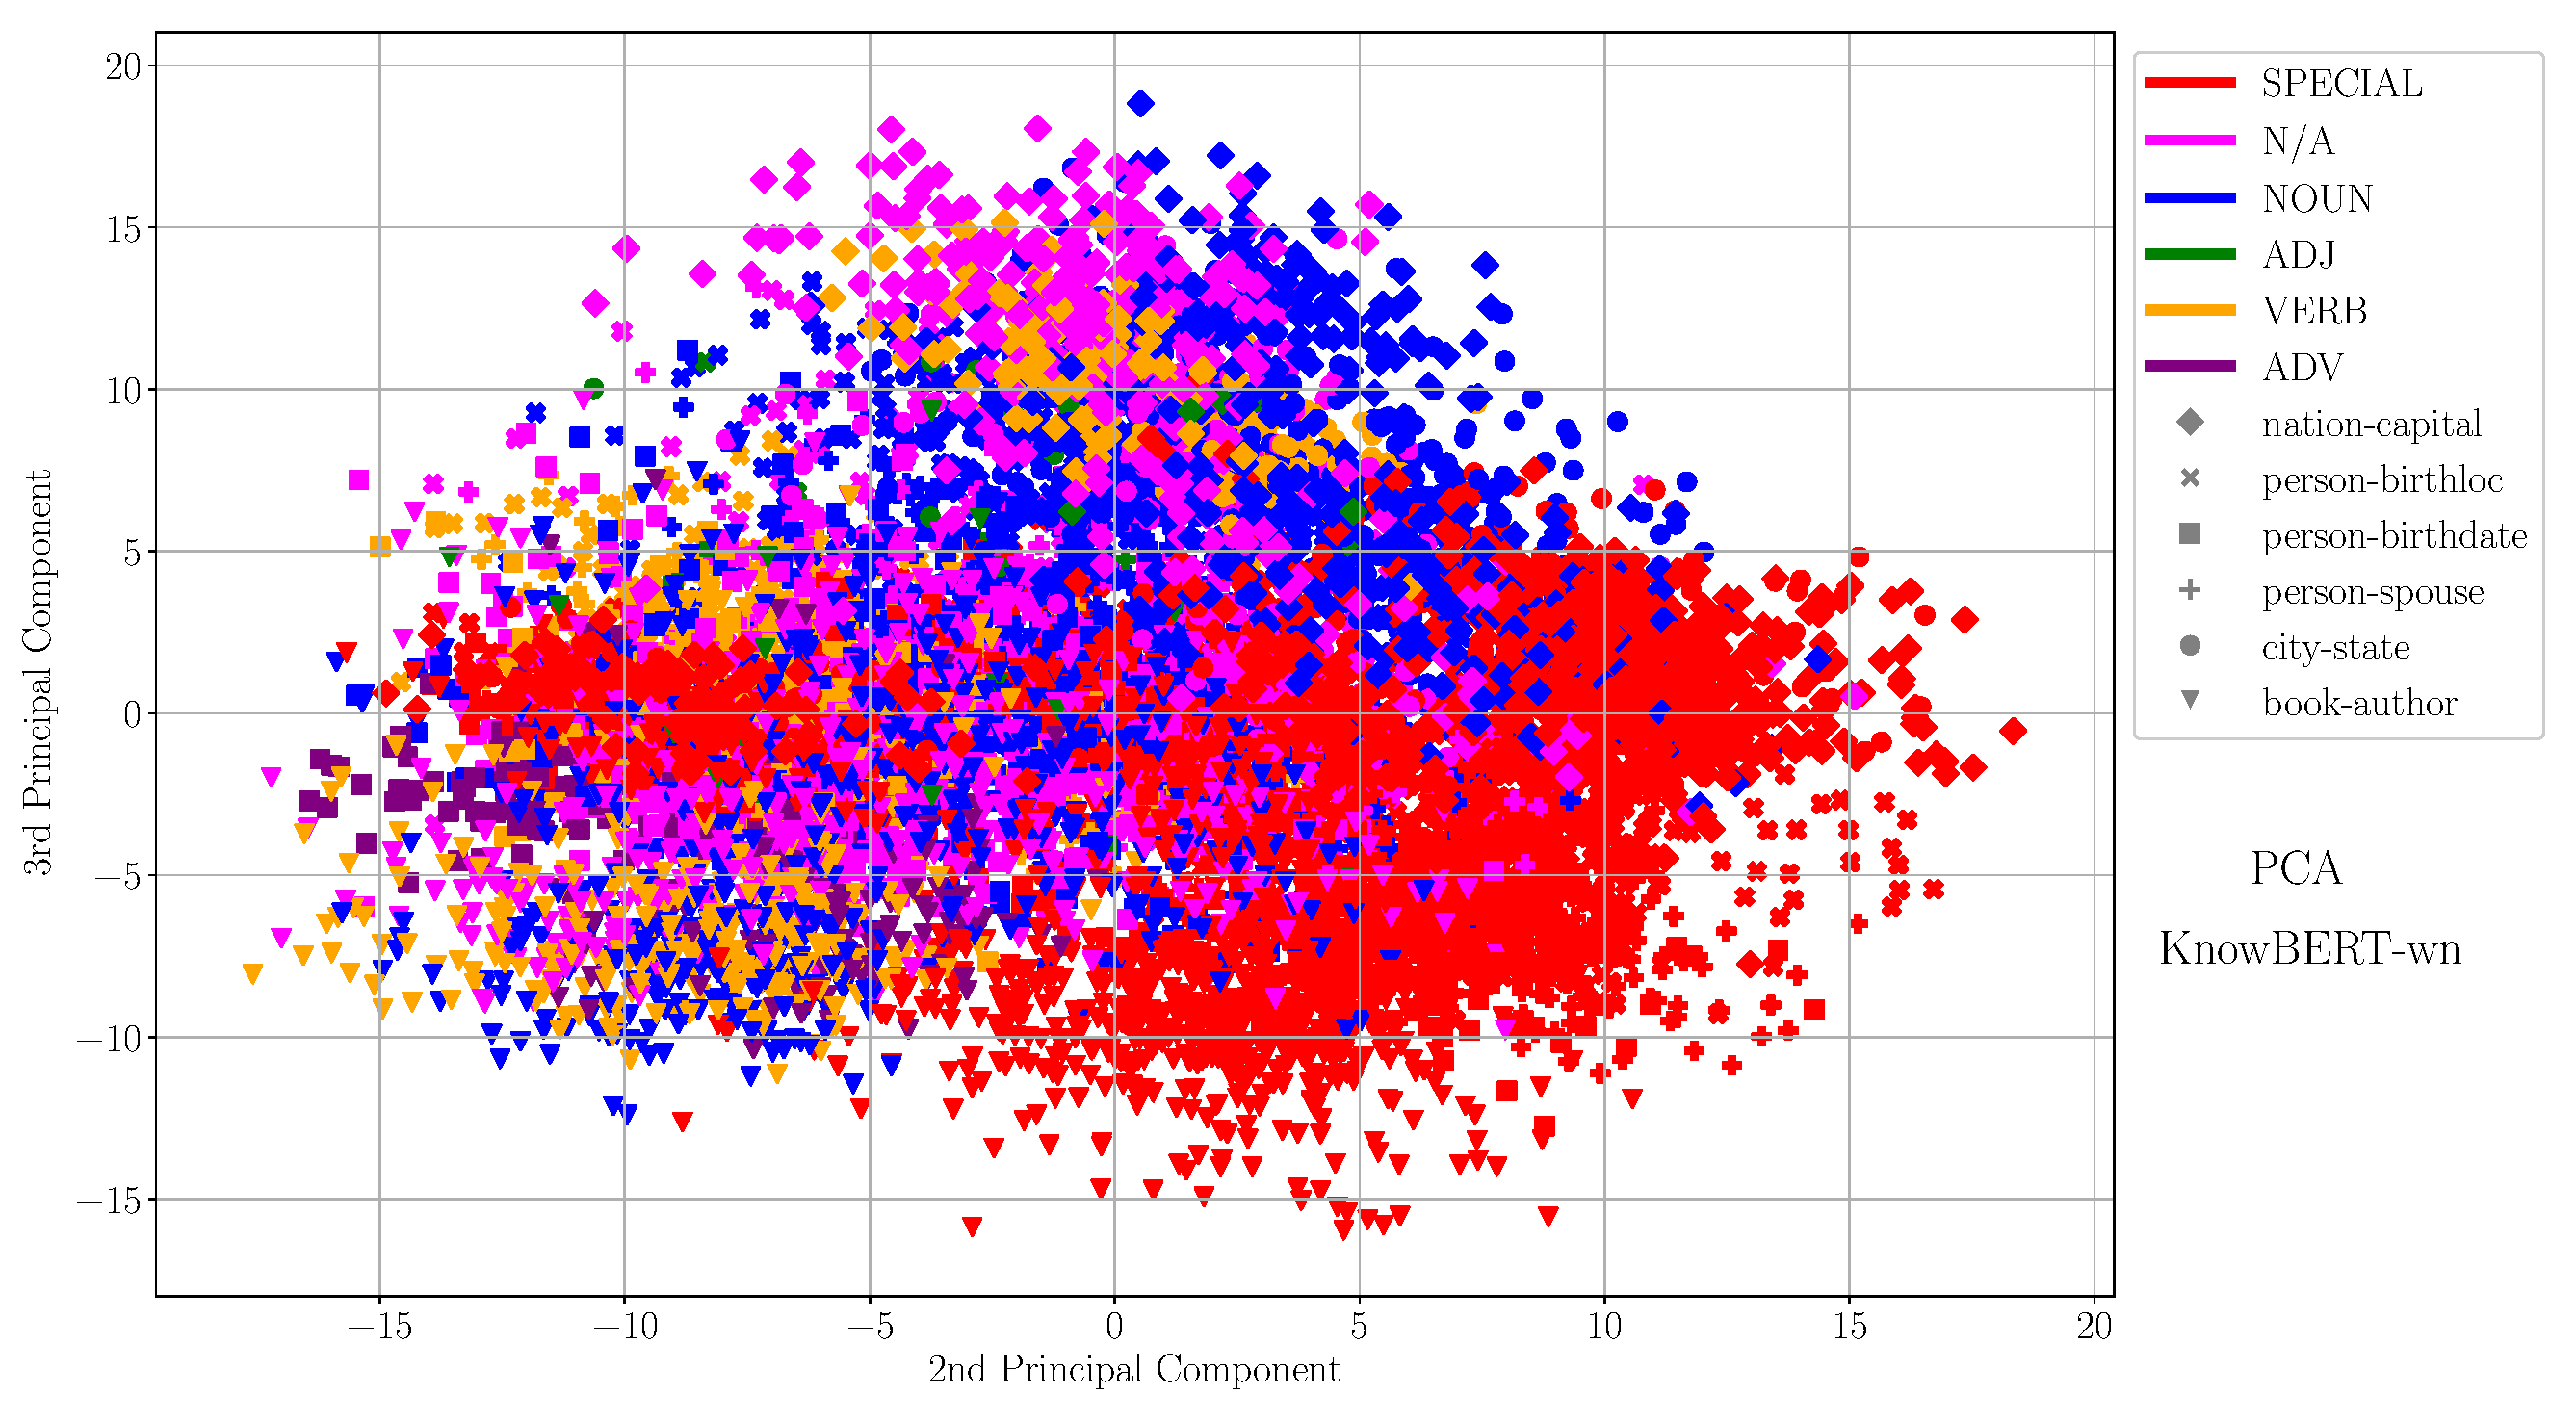
\includegraphics[height=0.15\textheight]{graphics/contextual_embeddings/PCA_9512_2_3_knowbert_wordnetNone_title.eps}
            \end{figure}
            \begin{figure}
                \centering
                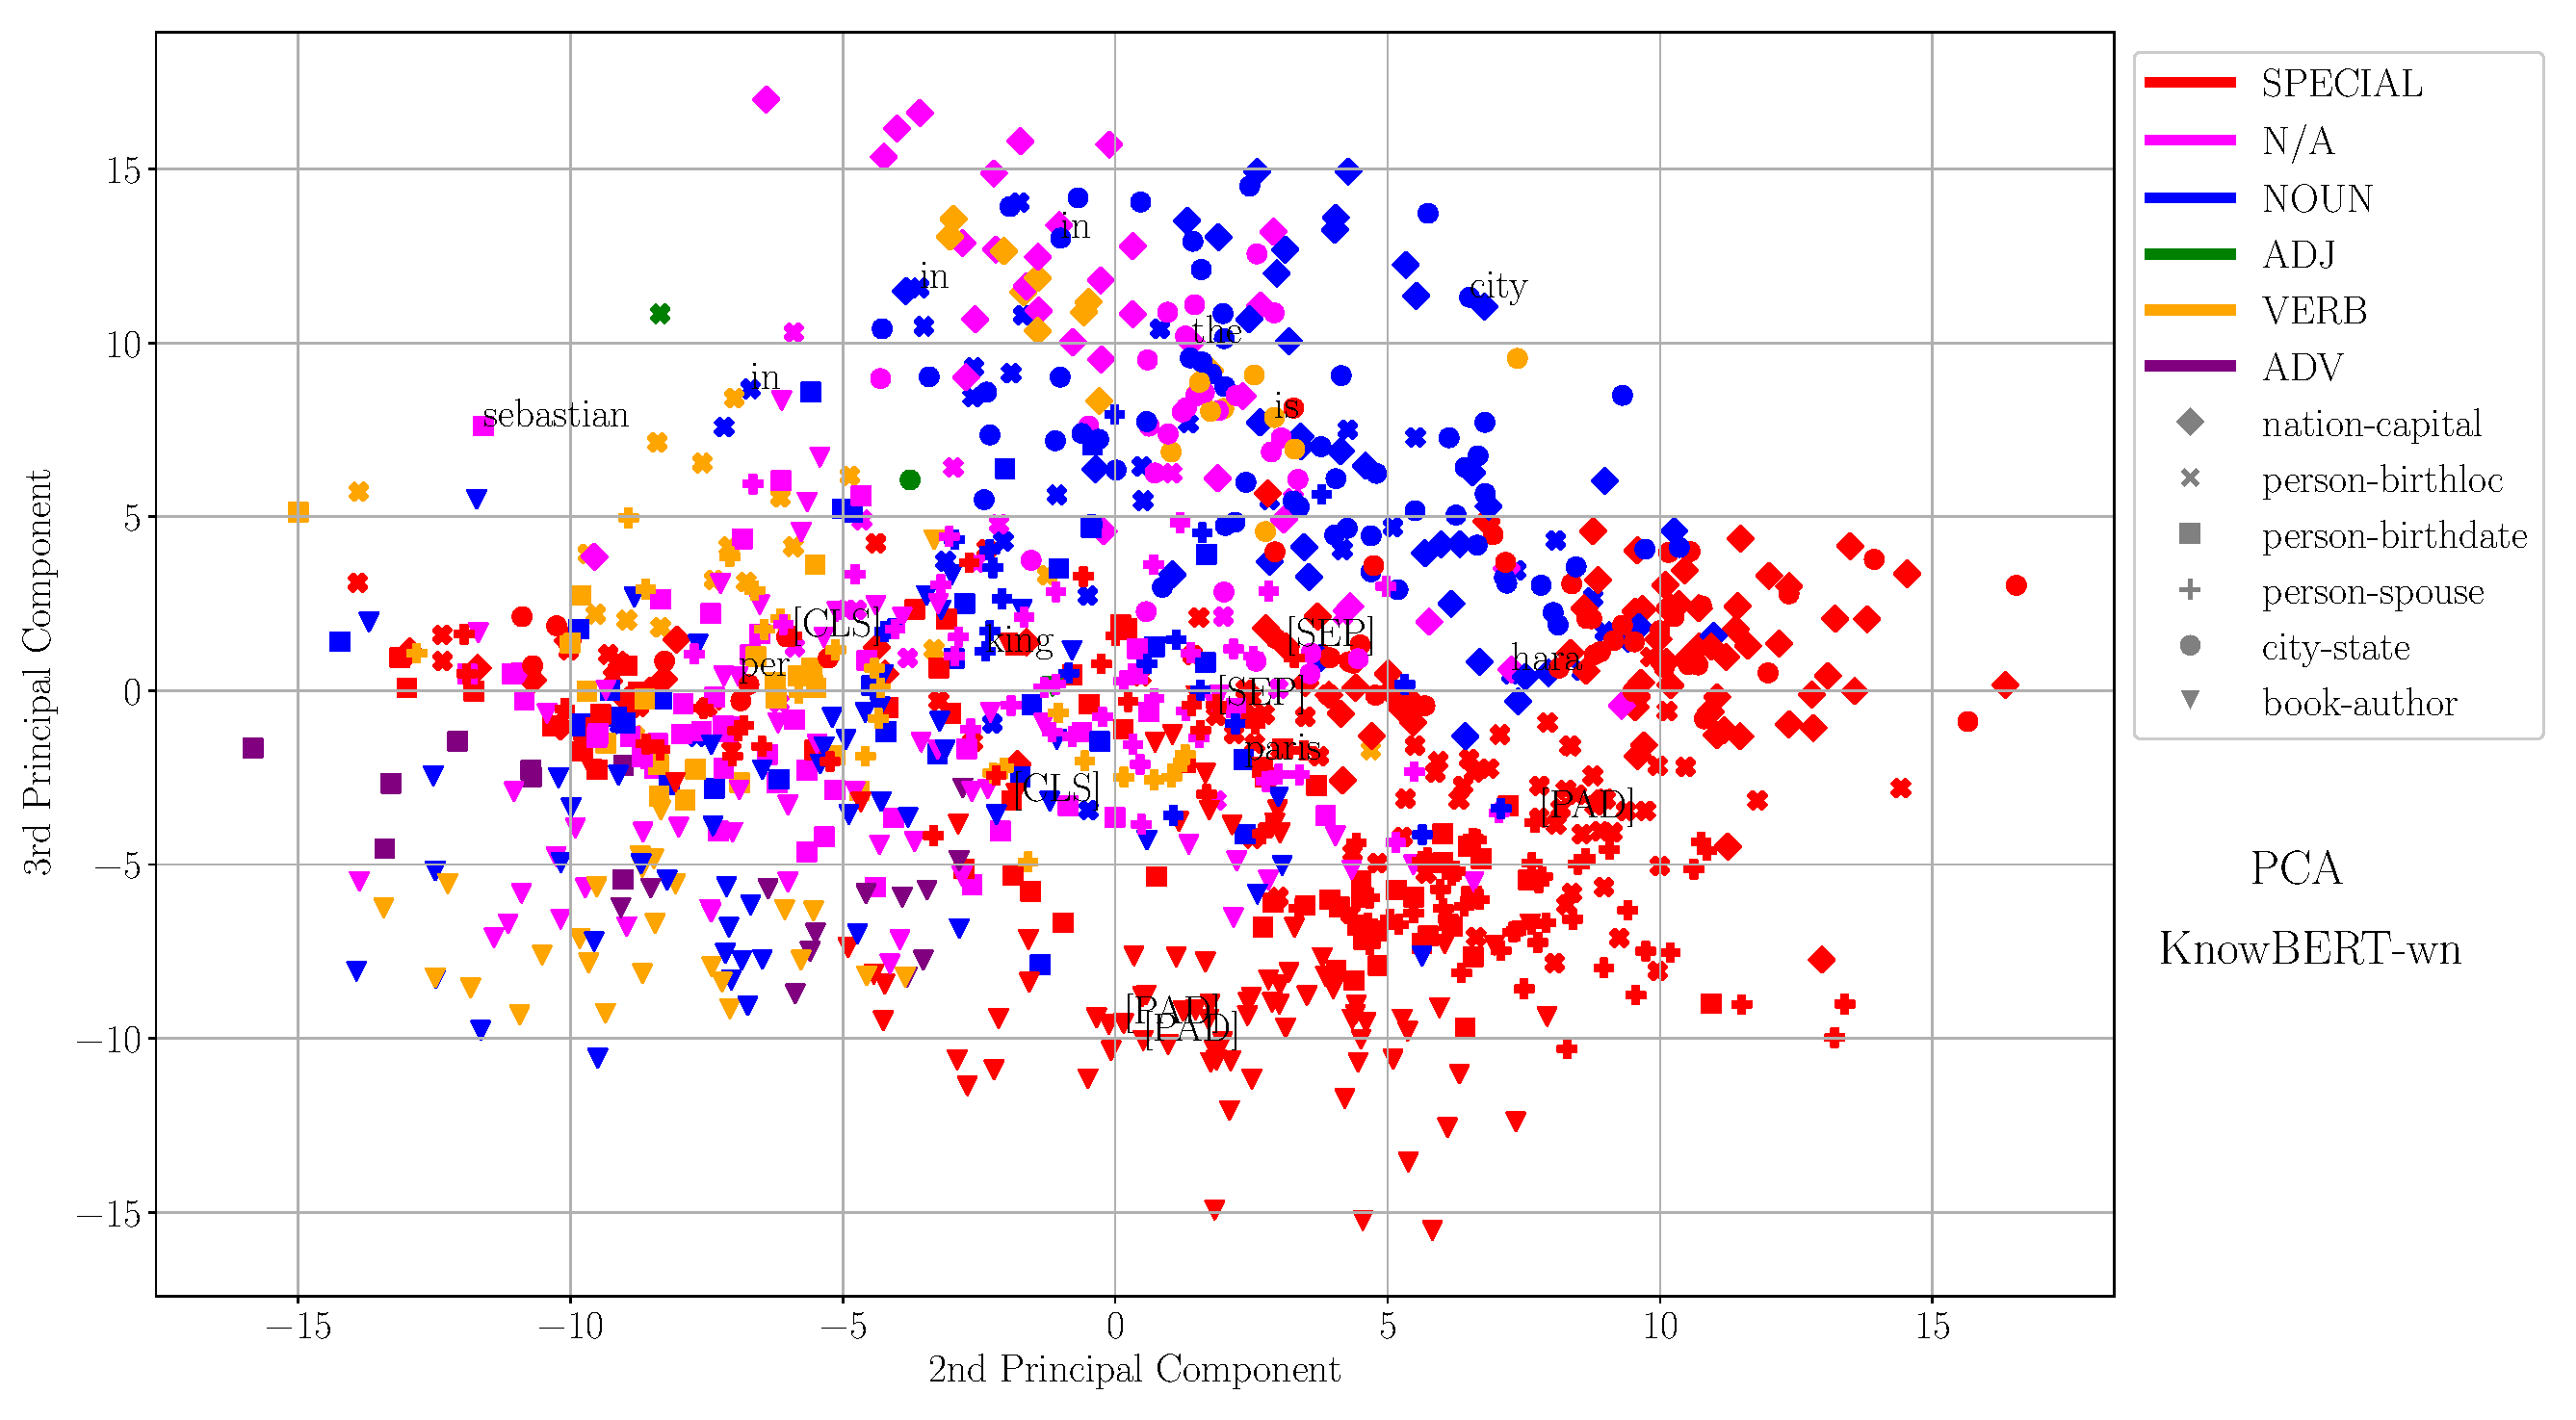
\includegraphics[height=0.55\textheight]{graphics/contextual_embeddings/PCA_1024_2_3_knowbert_wordnet_annotated_title.eps}
            \end{figure}
        \end{column}
        \begin{column}{0.5\textwidth}
        \textbf{KnowBERT-W+W}
            \begin{figure}
                \centering
                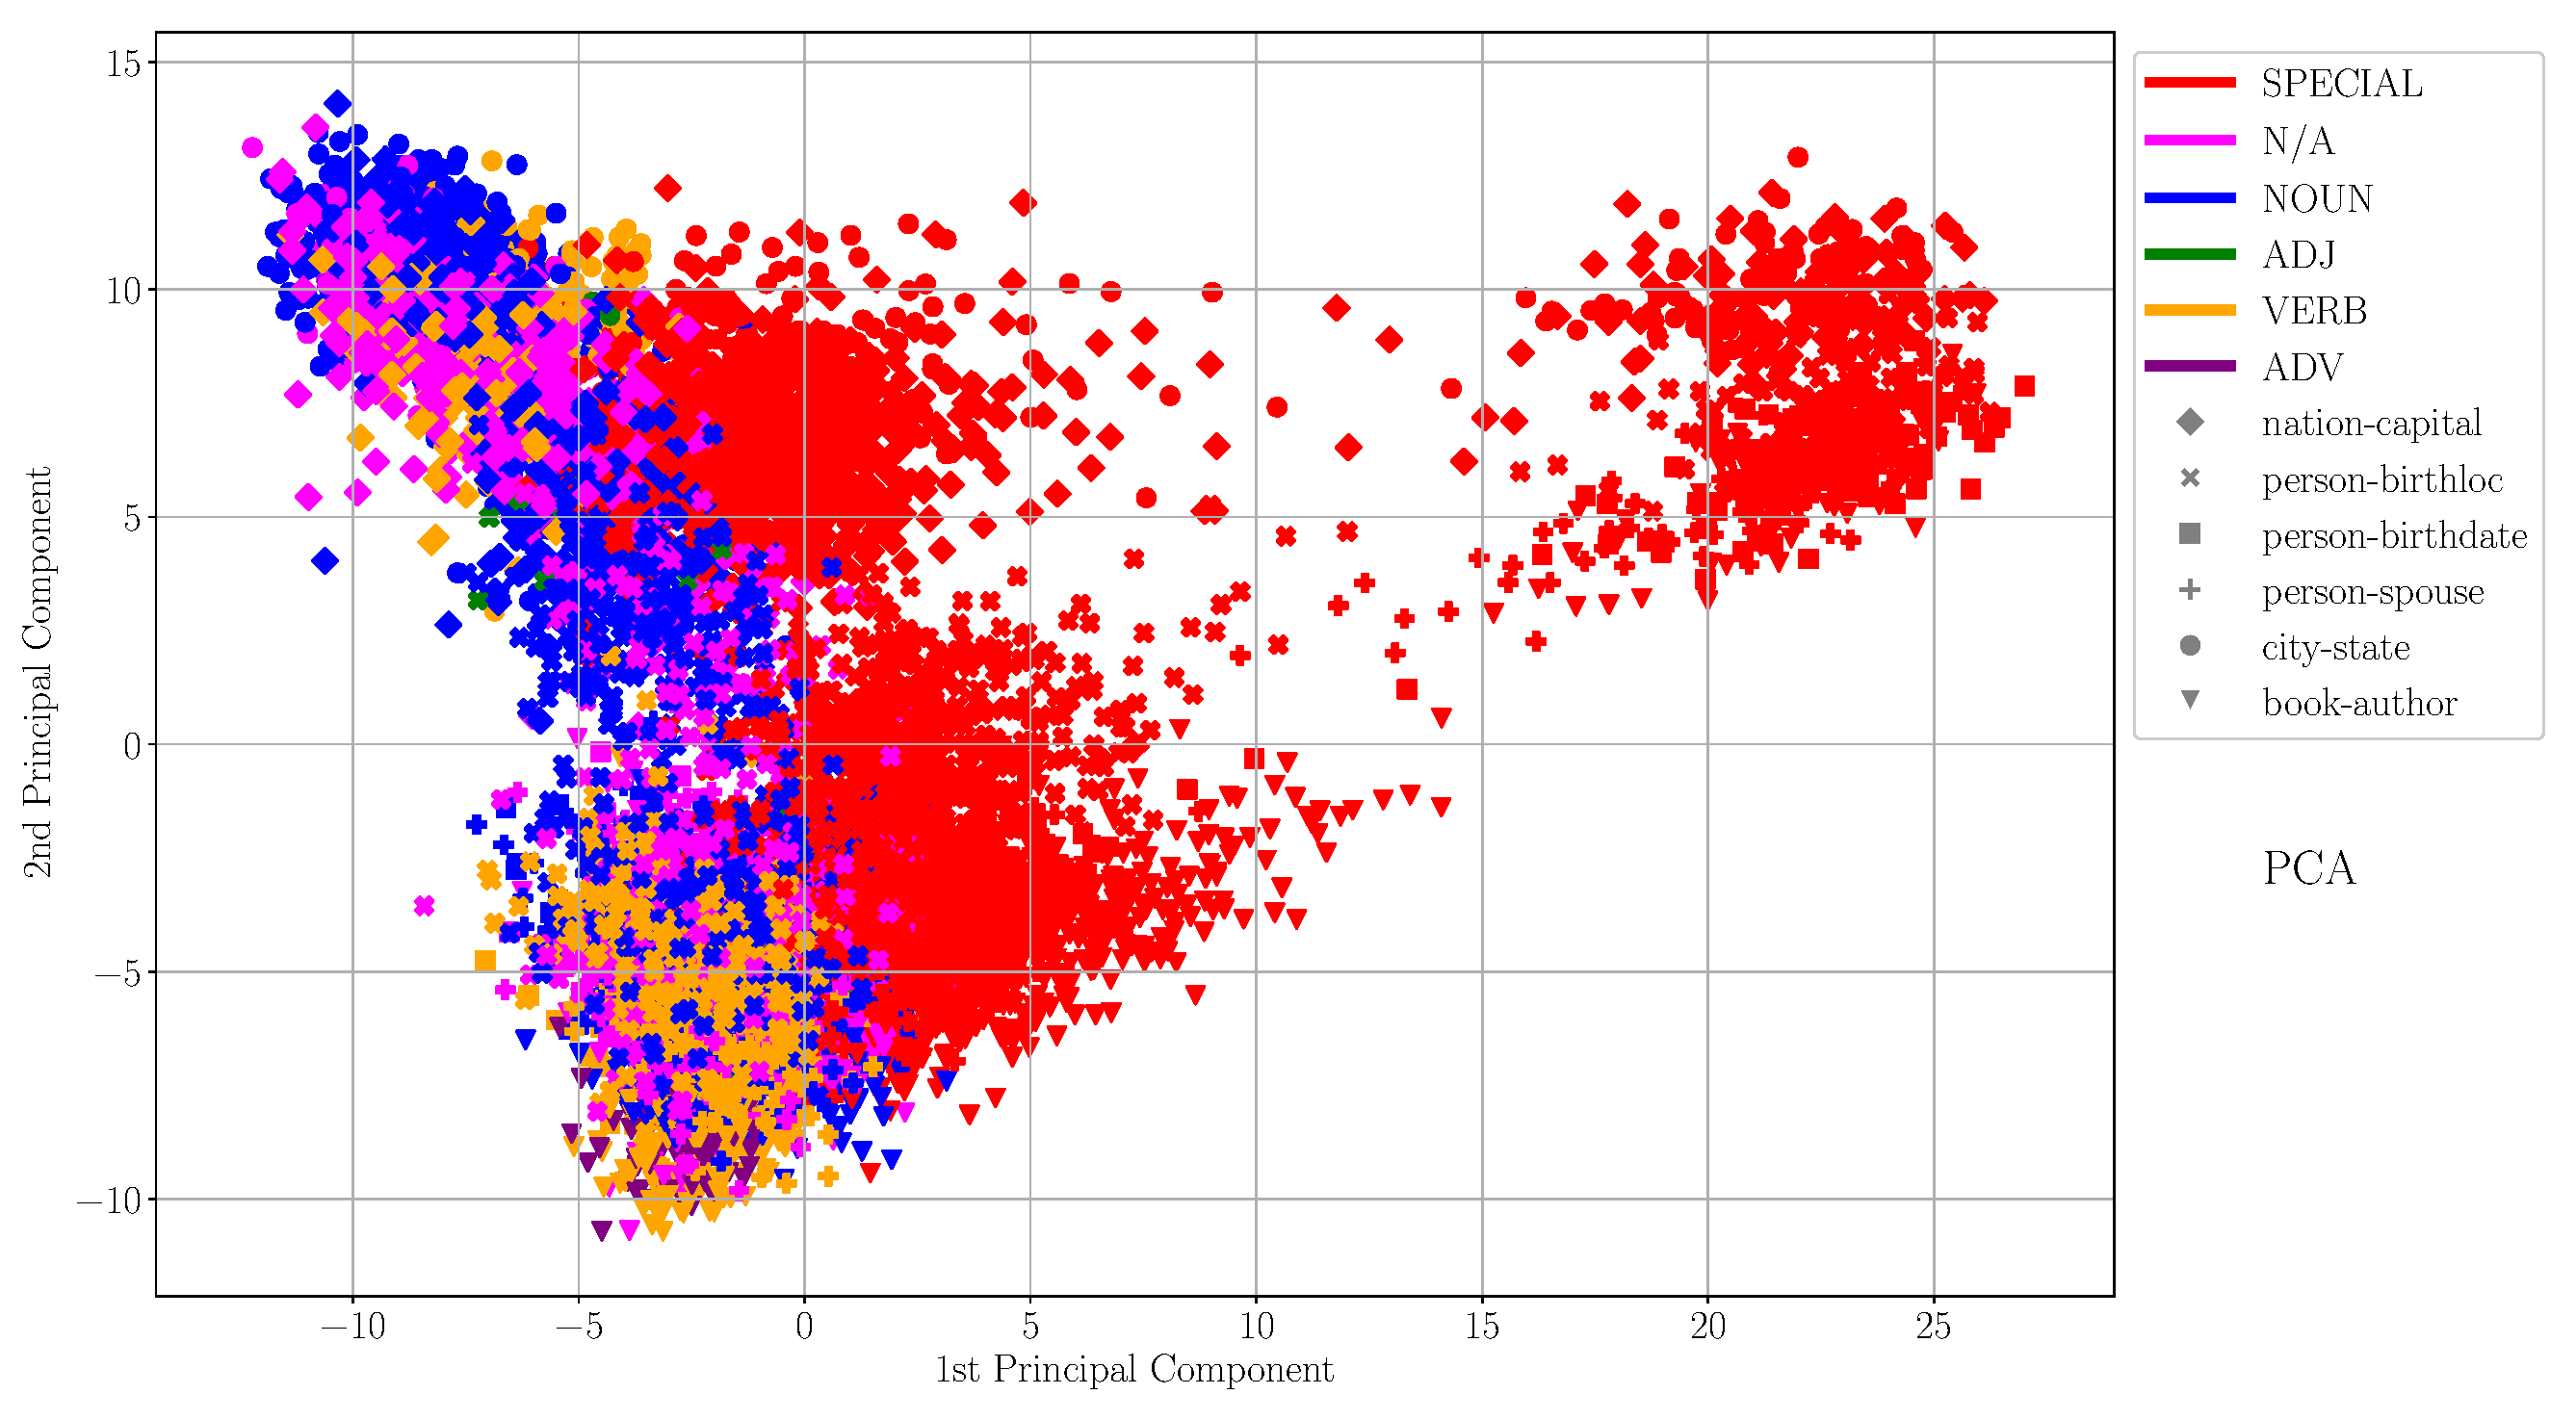
\includegraphics[height=0.15\textheight]{graphics/contextual_embeddings/PCA_9512_1_2_knowbert_wiki_wordnetNone_title_USE.eps}
            \end{figure}
            \begin{figure}
                \centering
                \includegraphics[height=0.55\textheight]{graphics/contextual_embeddings/PCA_400_1_2_knowbert_wikiwordnet_annotated_title_USE.eps}
            \end{figure}
        \end{column}
    \end{columns}
\end{frame}


% Recurring Observations
\begin{frame}{Recurring Observations: Contextual Embeddings compared to BERT-large}
\footnotesize
\colheading{DTU_red}{\begin{center}\textbf{All three KnowBERT variants}\end{center}}
\vspace{0.2cm}
\textbf{Similar to baseline:}
\begin{itemize}
    \item Classification tokens, [CLS], are projected to locations distant from the center projected onto 1st and 2nd PCs,
    \item Clear POS-tag related structures,
\end{itemize}
\textbf{Deviations from baseline:}
\begin{itemize}
    \item POS-tag clusters tend to be even more distinctive
    \begin{itemize}
        \item Especially regarding verbs,
    \end{itemize}
    \item Generally more dispersed, i.e., more variance per PC
\end{itemize}

\end{frame}



